\documentclass[12pt, oneside]{article}
\usepackage[margin=1in]{geometry}
\geometry{letterpaper}
%\geometry{landscape}
%\usepackage[parfill]{parskip}
\usepackage{graphicx}
\usepackage{amsmath}
\pagenumbering{arabic}		
\usepackage{amssymb}
\usepackage{pdfpages}
\usepackage{listings}
\usepackage{mathtools}
\usepackage[utf8]{inputenc}
\usepackage{float}
\usepackage{hyperref}


\title{STAT 243 Final Project\\Implementation of an Adaptive-Rejection Sampling Method}
\author{Ye Zhi, Boying Gong, Max Gardner, Alexander Brandt}
\date{December 17, 2015}

\DeclarePairedDelimiter\ceil{\lceil}{\rceil}
\DeclarePairedDelimiter\floor{\lfloor}{\rfloor}

\newcommand{\cpder}[3]{\left(\frac{\partial#1}{\partial#2}\right)_{#3}} %Constrained partial derivate
\newcommand{\pder}[2]{\left(\frac{\partial#1}{\partial#2}\right)} %Partial derivate
\newcommand{\dbar}{\ensuremath{\mathchar'26\mkern-12mu d}}
\newcommand{\nPr}[2]{ {_{#1}}P_{#2} } %Partial derivate

\begin{document}

\maketitle

\section{Project URL}

\url{https://github.com/boyinggong/243FinalProject}

\section{Theory}

Our final project was to implement an adaptive-rejection sampling method in R.  Our method largely implements the methods described by Gilks and Wild.  ARS attempts to efficiently generate random values according to a user-defined distribution (and a user-defined domain).  The method follows a few general steps, exploiting the tendency of many important and useful distributions to be log-concave (even if the distributions themselves are not concave).  For some distribution \(g(x)\), let us define \(h(x) = \log(g(x))\).  Note, this point, if \(h(x)\) is found to be not log-concave, then our program will reject the values.
\\\\
Now, in order to efficiently sample from values (and not waste time generating values that will ultimately be rejected), we construct an upper envelope function that bounds \(h(x)\).  This is performed by taking two or more starting points from within the domain such that they lie within our users defined bounds.  At points we will calculate the tangent's slope at \(x_i\).  We then calculate the x-intercept where these slopes meet with:
\[ z_j = \frac{h(x_{j+1}) - h(x_j) - x_{j+1}h'(x_{j+1}) + x_j h'(x_j)}{h'(x_j) - h'(x_{j+1})} \]
Where \(j \in [1,k-1]\).  Note that \(z_0\) and \(z_k\) are the upper and lower bounds of the function, respectively, even if those bounds are \(-\infty\) or \(\infty\).
\\\\
Now that we can define the envelope for \(x \in [z_{j-1}, z_j]\):
\[ u_k(x) = h(x_j) + (x - x_j)h'(x_j) \]
By exponentiating and normalizing this \(u_k(x)\), we now have a density from which to sample our random values:
\[ s_k(x) = \frac{\exp(u_k(x))}{N} \]
Where N is simply the all-space integral value of \(s_k(x)\) (i.e. \(N = \int_D s_k(x) dx \)).

Furthermore, we exploit a computationally inexpensive procedure to compute a lower hull, which is defined as:

\[ l_k(x) = \frac{(x_{j+1} - x)h(x_j) + (x - x_j) h(x_{j+1})}{x_{j+1} - x_{j}} \]

\(l_k(x) \) can allow us to perform a squeezing test to quickly accept or reject proposed sampling values.  This is performed by selecting some value \(x^t\) from \(s_k(x)\), and drawing a value \(w\) from the uniform distribution defined from [0,1].  We can accept \(x^t\) if:

\[ w \le \exp(l_k(x^t) - u_k(x^t)) \]

Or if:

\[ w \le \exp(h(x^t) - u_k(x^t)) \]

These are the squeezing test and rejection test, respectively.  As we continue to compute \(h(x^t\) and \(h'(x^t)\), we can update the points that construct our upper and lower hulls, thereby increasing the chance of new values drawn from \(s_k(x)\) being accepted.  This is the mathematical and statistical intuition behind the implementation discussed in the next section.

\section{Implementation}

In order to create a modular solution, we have created several helper functions in various files which are called by ars in ars.R in an order described above.  Our code was made modular, portable, and testable by use of functions that define each subroutine in the ARS calculation.

\begin{enumerate}

\item dh.R\\\\
Arguments: an x value to evaluate, a function \(g\)\\\\
Returns: \(g'(x)\)\\\\
The derivative of h is of critical importance throughout this procedure.  To implement, we use a dh method that takes advantage of numerical derivation (via numericDeriv in the stats package) to find our tangents.\\

\item find\_init.R\\\\
Arguments: a function \(g\), and a list specifying the range it is defined on\\\
Returns: a list of two entries corresponding to the left and right starting hull \(x_i\)'s.\\\\
Though it would always be best for the user, who has a better understanding of the distribution, to supply their initial points, it was our intention that the program perform well even in cases when the user did not.  To this end, ars.R begins by calling find\_init.R\\

\item get\_zj.R\\\\
Arguments: x values of hull points, y values (h(x)'s) of hull points, slope of the hull points\\\\
Returns: a list of all intersection points (\(z_j\)'s)\\\\
To compute the intersection between our tangents, we use get\_zj.R.  It computes all the intersections given various \(x_i\)'s from the formula given above.\\

\item upper\_piecewise.R\\\\
Arguments: an x to evaluate, the x values of hull points, y values (h(x)'s) of hull points, slope of the hull points, and the total domain of the probability distribution function\\\\
Returns: u(x)\\\\
This uses a vectorized formulation to compute \(u(x)\) by using a boolean operation based on \(x\)'s range, the range of \(z_i\), to compute the correct piece (i.e. only the relevant line segment for a given range will be used to compete \(u(x)\).

\item lower\_piecewise.R\\\\
Arguments: an x to evaluate, the x values of hull points, y values (h(x)'s) of hull points, and the total domain of the probability distribution function\\\\
Returns: l(x)\\\\
This uses a vectorized formulation to compute \(l(x)\) by using a boolean operation based on \(x\)'s range, the range of \(z_i\), to compute the correct piece (i.e. only the relevant line segment for a given range will be used to compete \(l(x)\).  (The only difference is that this is the lower chord hull, and that for points between the domains an the first and last \(x_i\), a large negative number returned as the constant value.

\item sk.R\\\\
Arguments: the x values of hull points, y values (h(x)'s) of hull points, and the total domain of the probability distribution function\\\\
Returns: a list of the non-normalized integral values of each piecewise exponential\\\\
Takes advantage of an explicit form of the inverse cumulative distribution function for an exponential (given that all \(u(x)\) are linear, and thus the integral of \(\exp(u(x))\) can be computed explicitly (i.e. without use of any integration packages).\\

\end{enumerate}

From here, we sample using \(s_k(x)\).  The procedure, as implemented, is fairly straightforward.  To begin, we select one of the pieces of the piecewise exponential probability distribution function by normalizing the curve, drawing a random value from the uniform distribution on [0, 1], and choosing the largest segment index such that the total integral value from the lowest domain to that region's upper bound is greater than the randomly drawn value.  Then, based on the normalized sub-region we sample a value \(x^t\) using the inverse CDF for the exponential (again, this can be explicitly solved), using another random variable \(u\) drawn from the uniform distribution on [0, 1].  More explicitly:

\[ u = \int_{z_i}^{x^t} exp(k_i (x - x_i) + y_i) dx = \left. \frac{exp(k (x - x_i )+ y_i)}{k} \right|_{z_i}^{x^t} \] 

Where \(u\) is our randomly generated number, \(x_i\), \(y_i\), and \(k_i\) are the x value, y value, and slope of the hull point, and \(z_i\) is the lower bound of the region of the piecewise exponential we are drawing from.  This value can then be accepted or rejected using the squeezing or rejection tests which is the final step implemented by ars.R.    A limit is also placed on how many hull points can exist for a given simulation.  Once we have selected enough values (as defined by the user), we return the array of numbers.

\section{Testing}

Boying fills this in.

\section{Results/Examples}

We provide some basic results in addition to the extensive testing of each function individually, which can be seen in more detail in the test suite defined in the package.

\subsection{Normal Distribution}

\begin{figure}[H]
\centering
  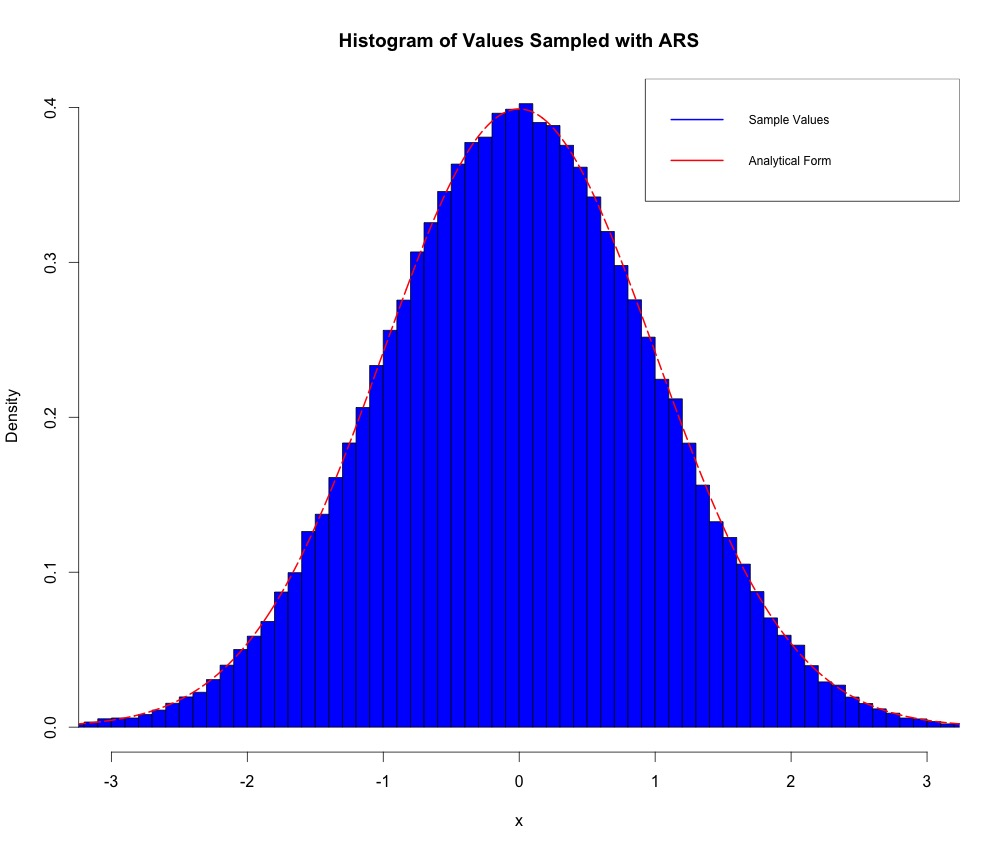
\includegraphics[scale=.25]{figure/normal.jpeg}
  \caption{The Normal Distribution.}
  \label{fig:d1}
\end{figure}

\subsection{Chi-Squared Distribution}

\begin{figure}[H]
\centering
  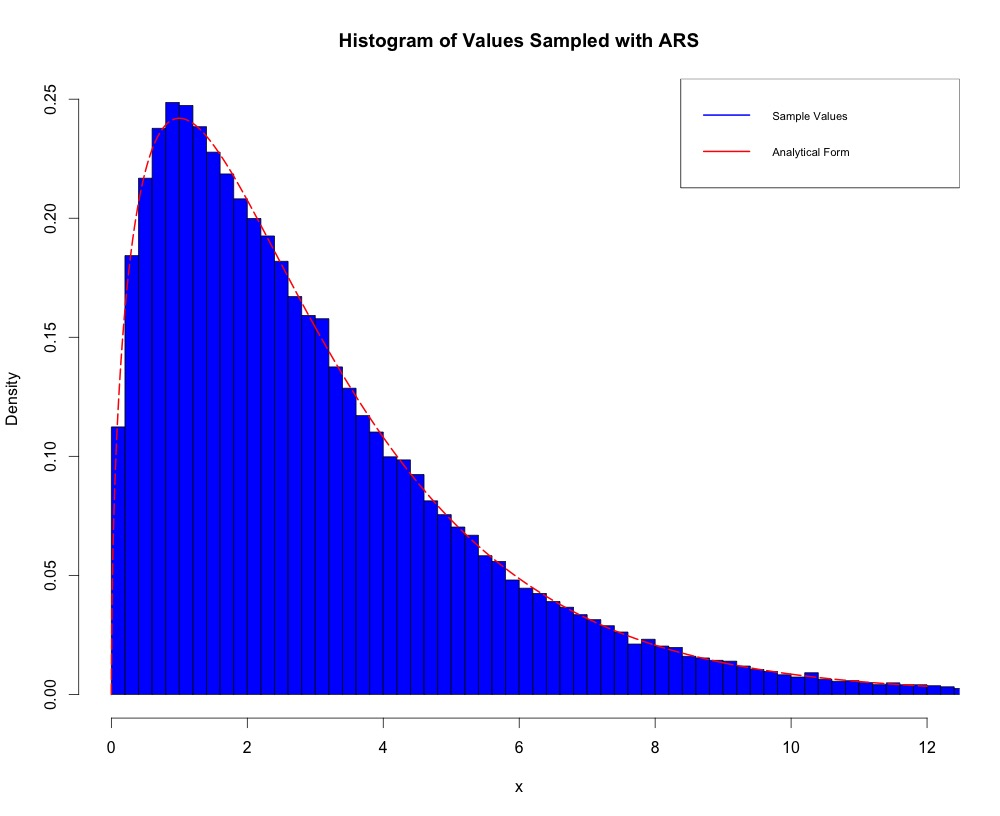
\includegraphics[scale=.25]{figure/chi_squared_dof3.jpeg}
  \caption{The Chi-Squared Distribution with 3 Degrees of Freedom}
  \label{fig:d2}
\end{figure}

\subsection{Uniform Distribution}

\begin{figure}[H]
\centering
  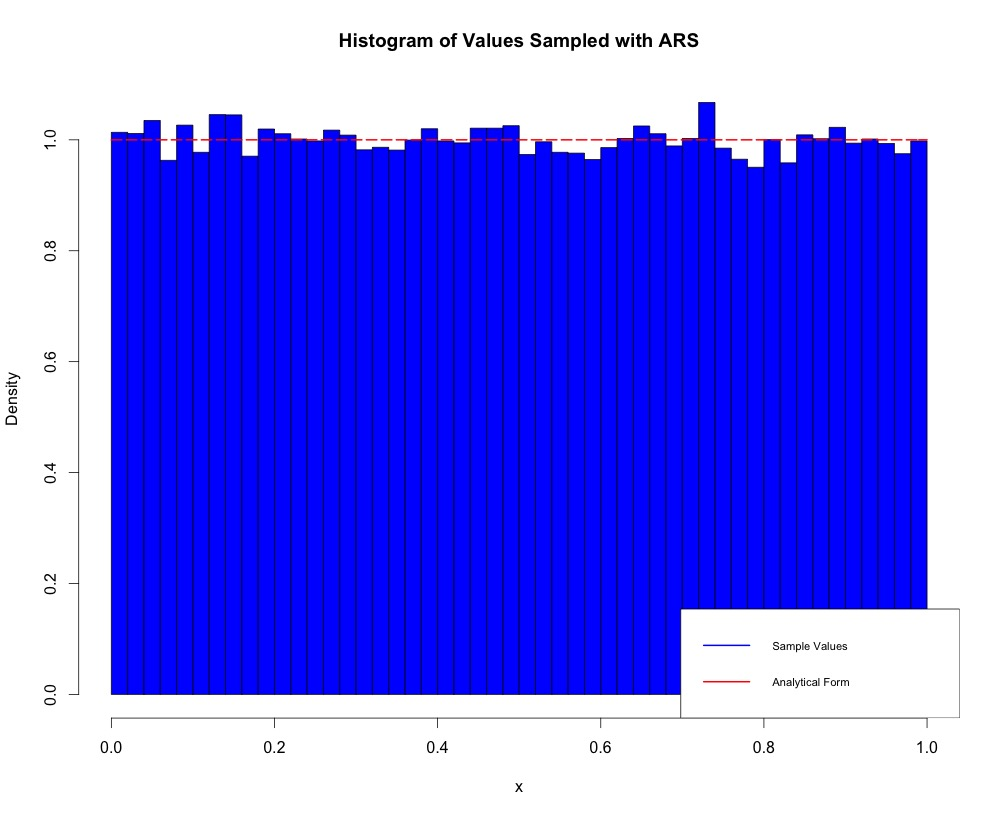
\includegraphics[scale=.25]{figure/uniform.jpeg}
  \caption{The Uniform Distribution on [0,1]}
  \label{fig:d3}
\end{figure}

\subsection{Exponential Distribution}

\begin{figure}[H]
\centering
  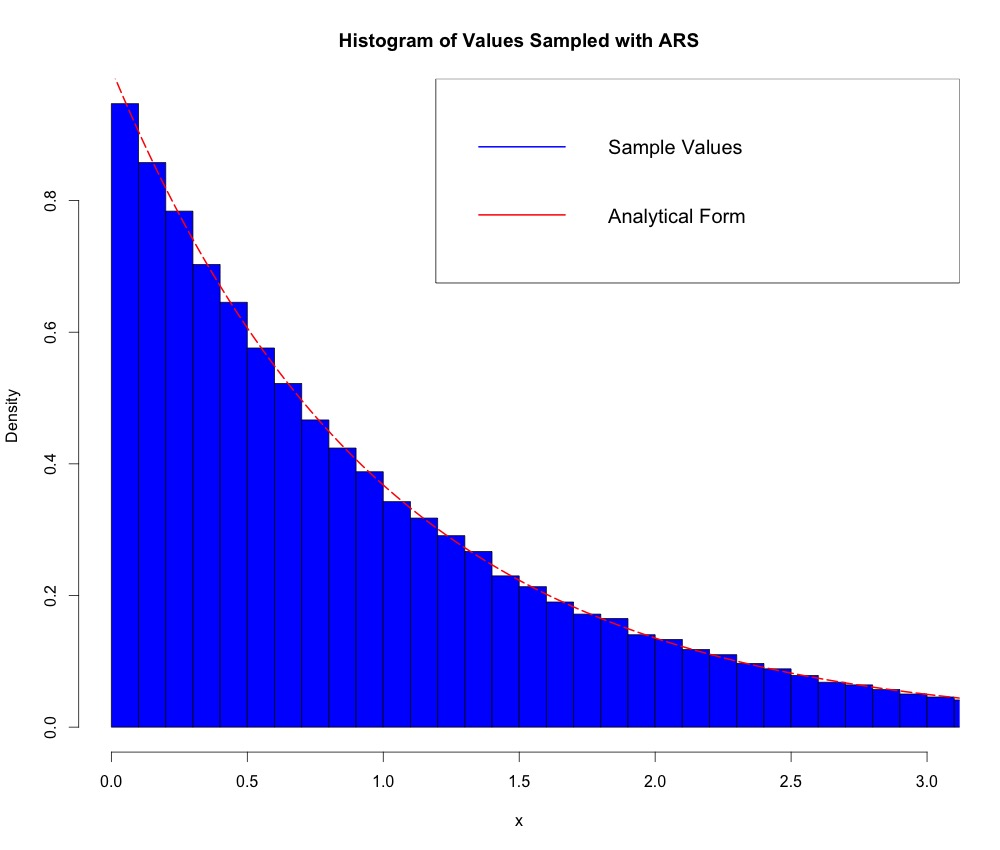
\includegraphics[scale=.25]{figure/exponential.jpeg}
  \caption{The Exponential Distribution, with \(\lambda = 1\).}
  \label{fig:d3}
\end{figure}

\section{Roll the Credits}

Ye Zhi \\\\
Boying Gong \\\\
Max Gardner developed auxillary functions for ARS, lead the documentation effort, and rolled everything up into a nice and neat R package. He is a first-year MS/PhD student in Civil Systems.\\\\
Alexander Brandt wrote an initial implementation of the ARS and \LaTeX'd up the final report.  He is a computational biologist interested in worms, humans, and what they have in common (and what they don't!).\\

\section{Citations}
1. Gilks, W. R., and P. Wild. ``Adaptive Rejection Sampling for Gibbs Sampling''. Journal of the Royal Statistical Society. Series C (Applied Statistics) 41.2 (1992): 337--348.\\\\
2. Wild, P., and Gilks, W. R.  ``Algorithm AS 287: Adaptive Rejection Sampling from Log-Concave Density Functions''. Journal of the Royal Statistical Society. Series C (Applied Statistics) 42.4 (1993): 701--709.



\end{document}